\section{Evaluation}
\label{sec:results}

Using linguistic definitions, we identified barks with natural language characteristics and distinct minimal sound units from canine vocalizations, which we define as words and phonemes in the canine vocalization communication system. To validate the effectiveness of the phonetic alphabet, we observed and listened to the audio samples of merged phones and manually verified the consistency within phonemes and the differences between phonemes. To verify the correctness of the word list, we randomly sampled videos of the 41 most frequent words and had their meanings judged by humans, ultimately obtaining relatively stable meanings for each word.

\subsection{Setup}

\begin{table}[th]
\centering
\small
\begin{tabular}{lll}
\hline
\textbf{Type} & \textbf{Labels}\\
\hline
\verb|Dog| & 1-3, 5-9, 11-19, 21, 22, 25-31, 33-36, 40-49, 51, 55-64, \\
& 66-70, 73-77, 80, 81, 83, 84, 86, 88, 90-107, 110-113, \\
& 115-118, 121, 123-133, 135, 136, 138, 139 \\
\verb|Noise| & 4, 10, 20, 23, 24, 32, 37, 39, 50, 52, 53, 54, 65, 71, \\
& 72, 78, 79, 82, 85, 87, 89, 108, 109, 114, 119, 120, \\
& 122, 134, 137 \\\hline
\end{tabular}
\caption{Dog phones vs noice phones before the iteration.}
\label{tab:phoneclassification}
\end{table}

After representing each sentence we have in the canine corpus, we totally have 140 different phones. For preliminary evaluating the quality of phones, we sample 10 samples of each phone and judge if it is a dog back. And we find there are 29 phones are noise like background noise, the crush sound of claw and 111 phones are dog vocalizations as shown in \tabref{tab:phoneclassification}. 

There are two hyper parameters in our phoneme finding algorithm, the minimal frequency of valid words and the KL divergence threshold for merging phones. The first parameter determines which words are qualified be considered ``word candidate'', the second parameter determines how similar the context two words hold, we are gonna to merge them together. We tried 1, 3 and 5 on minimal frequency of valid words and 5, 10, 15 on KL divergence threshold. We finally pick up 5 and 15 percentile to be the hyper parameters respectively.

\subsection{Results}

\begin{table}[th]
\centering
\small
\begin{tabular}{lll}
\hline
\textbf{Type} & \textbf{Labels}\\
\hline
\verb|Phonemes| & 6, 1, 15, 12, 28, 74, 4, 42, 130, 95, 92, 39, 87, 2, 8, \\
& 107, 23, 93, 126, 30, 88, 96, 80, 3, 22, 135, 73, 51, \\
&137, 129, 70, 90, 66, 136, 21 \\\hline
\end{tabular}
\caption{Phoneme Alphabet}
\label{tab:pa}
\end{table}

\begin{table}[th]
\centering
\small
\begin{tabular}{lll}
\hline
\textbf{Phoneme} & \textbf{Phones to be merged}\\
\hline
\verb|1| & 11, 17, 18, 48, 86, 104  \\
\verb|2| & 97 \\
\verb|6| & 7, 9, 14, 16, 25, 33, 46, 57, 115, 127 \\
\verb|12| & 43, 83, 124 \\
\verb|15| & 31, 61, 77, 99, 110, 123, 125 \\
\verb|28| &59, 113, 116 \\\hline
\end{tabular}
\caption{Merged Phones}
\label{tab:mp}
\end{table}

The phoneme we finally have is shown in \tabref{tab:pa} which consist of 30 dog vocalization phonemes and 5 noise phonemes. Other 20 noise phones are automatically eliminated by the phoneme finding algorithm and 4 noise phones are eliminated by word segmentation. Testers also hear the randomly selected samples of merged phones as shown in \tabref{tab:mp}, the sound patterns are generally the same, but there are differences in timbre, volume, and other sound effects among the samples. However, it can be determined that they can be classified into the same category.

\begin{table}[th]
\centering
\small
\begin{tabular}{lclc}
\hline
\textbf{Words} & \textbf{Frequency} & \textbf{Words} & \textbf{Frequency}\\
\hline
\verb|28 12 6 15| & 1110 & \verb|28 12 1| & 996 \\
\verb|28 12 6| & 927 & \verb|28 12 6 1| & 828 \\
\verb|28 12 1 15| & 826 & \verb|28 12 15| & 706 \\
\verb|28 12 6 1 15| & 513 & \verb|28 6| & 452 \\
\verb|6| & 378 & \verb|12 6| & 303 \\
\verb|12 6 1| & 291 & \verb|28 6 15| & 274 \\
\verb|126| & 270 & \verb|135| & 261 \\
\verb|28 15| & 251 & \verb|28 12| & 248 \\
\verb|12 6 15| & 197 & \verb|12 1| & 180 \\
\verb|12 15| & 172 & \verb|42 51| & 162 \\
\verb|95| & 153 & \verb|28 74 130| & 149 \\
\verb|28 93 107| & 146 & \verb|28 6 1| & 144 \\
\verb|28 12 1 2| & 144 & \verb|6 15| & 140 \\
\verb|28 12 6 1 6| & 138 & \verb|93| & 135 \\
\verb|51 22| & 135 & \verb|28 12 130| & 129 \\
\verb|28 74 12 15| & 122 & \verb|51| & 117 \\
\verb|136| & 117 & \verb|129| & 117 \\
\verb|28 12 1 6| & 117 & \verb|28 12 95| & 114 \\
\verb|80| & 108 & \verb|6 3| & 108 \\
\verb|28 74 15| & 107 & \verb|28 126| & 106 \\\hline
\end{tabular}
\caption{Most frequent words and its frequency}
\label{tab:mfw}
\end{table}

The selected word list we find is shown in \tabref{tab:mfw}. We totally find 278 different words from the corpus and 204 of them are purely dog words with any noise phoneme. From the table, we can see that the word "28-12-6" appears frequently because many phones have been replaced with the phonemes in this word, and there is no overlap between these words. We believe that this combination of phonemes is likely a fixed pattern in canine language.

\subsection{Phonemes Evaluation}

By continuously merging word pairs with similar environments (lower KL divergence) and differing by only one phoneme, we gradually obtained the final phonetic alphabet with 35 phonemes. This process is illustrated in the \figref{fig:clusters}, where each iteration involves replacing a phone with a similar phone, ultimately resulting in a sparser phoneme distribution. In each iteration, our proposed algorithm first iteratively identifies all minimal pairs in the corpus, as shown in the \tabref{tab:mps}. We then retain only the words that contain phonemes with minimal pairs and use these words to generate the next iteration's phone list. This process continues until all phones are included in minimal pairs.

Moreover, the algorithm automatically removes noisy phones from the transcription through continuous iteration and refinement, indirectly demonstrating its ability to retain phones with specific patterns in canine vocalizations and the potential to uncover meaningful information.

\begin{figure*}[h]
    \centering
    \scalebox{0.17}{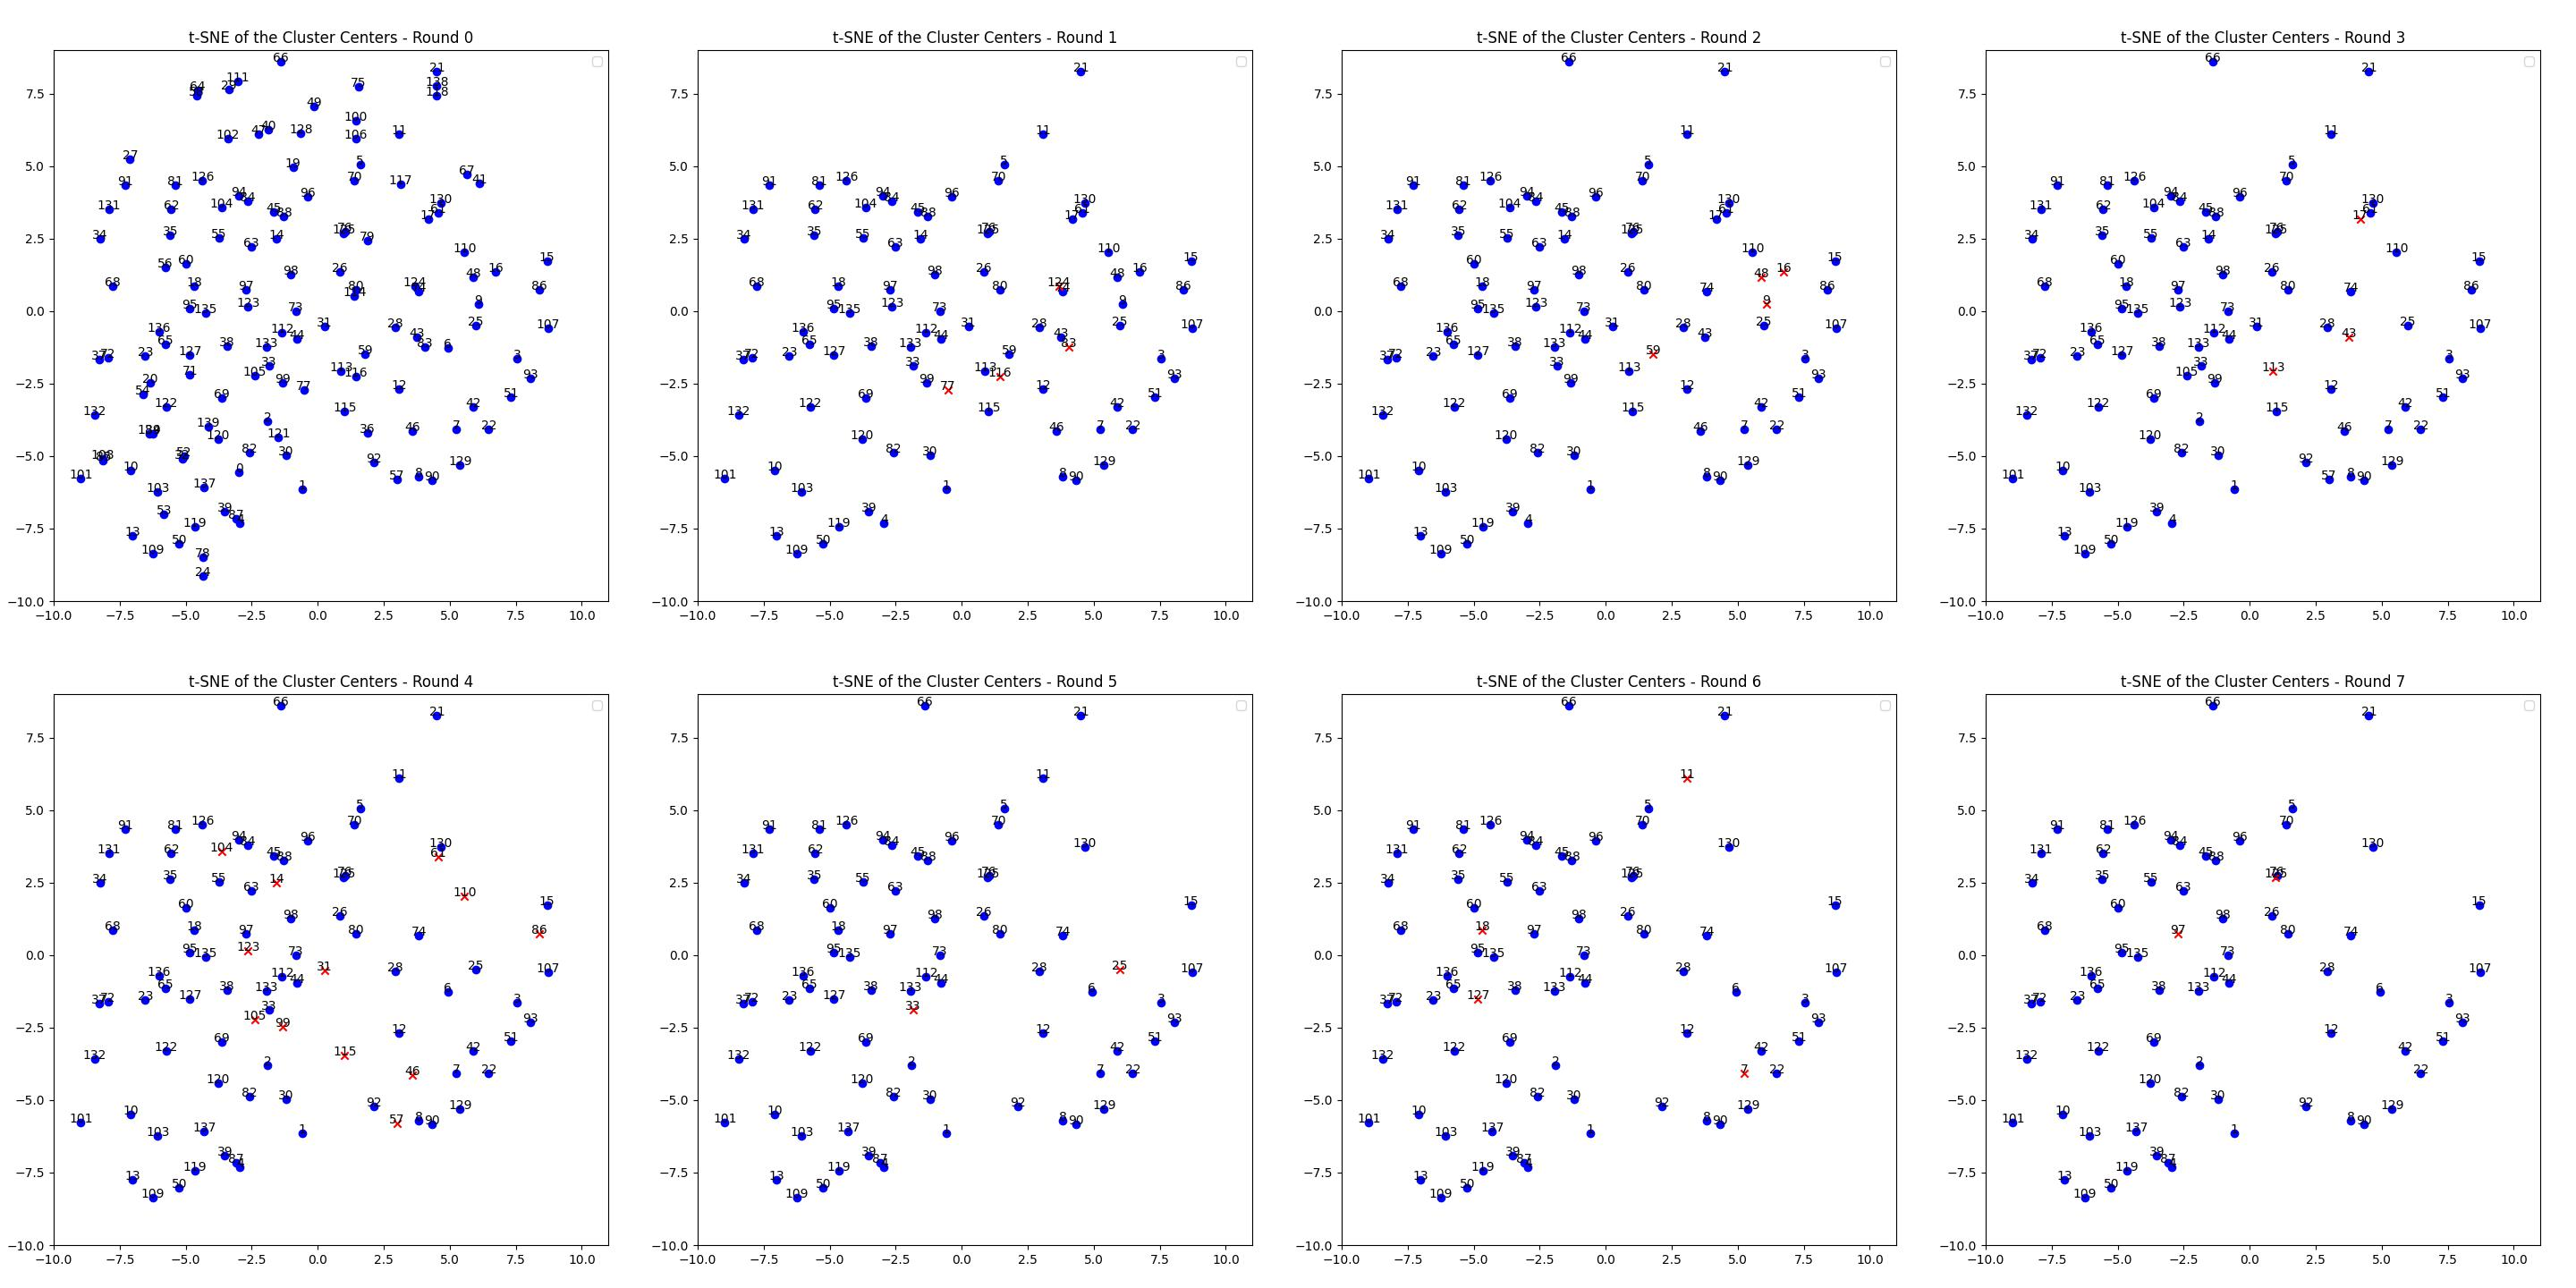
\includegraphics{images/phone_merging_image.jpg}}
    \caption{Changes in phone distribution after each iteration.}
    \label{fig:clusters}
\end{figure*}

\begin{table}[th]
\centering
\small
\begin{tabular}{lll}
\hline
\textbf{Phone Pair} & \textbf{Context}\\
\hline
\verb|6, 12| & (4 28 6 1) vs (4 28 12 1)  \\
\verb|12, 74| & (28 12 15 2) vs (28 74 15 2) \\
\verb|4, 39| & (4 28 6) vs (39 28 6) \\
\verb|6, 28| & (6 12 6) vs (28 12 6) \\
\verb|6, 4| &(6 12 6) vs (4 12 6) \\\hline
\end{tabular}
\caption{Minimal Pair Samples}
\label{tab:mps}
\end{table}

\paragraph{Human Evaluation}

\begin{table}[th]
\centering
\small
\begin{tabular}{lc}
\hline
\textbf{Tester} & \textbf{Accuracy}\\
\hline
\verb|Tester 1| & 64.00\%  \\
\verb|Tester 2| & 69.67\%  \\
\verb|Tester 3| & 68.67\% \\
% \verb|Tester 3| & AudioSep & \pmb{0.7755} \\
\verb|Agreement| & 74.22\%  \\\hline
\end{tabular}
\caption{Accuracy and agreement result on testing the reliability of phonemes discovery}

\label{tab:phonetestresult}
\end{table}

A phoneme, as a distinct sound unit that can distinguish one dog word from another, it is important to hold a consistency within the same phoneme and difference between two different phonemes. Especially after we merged few phones together. For evaluating these two properties, we let testers determine the sample pairs in the same phoneme or cross the phonemes if the same. For in-phoneme pair, we totally sampled 5 pairs for each phoneme, for cross phoneme pairs, we also randomly select 175 pairs. There are total 350 pairs of phoneme samples. Testers are required to label they are the same or not. The result is shown in \tabref{tab:phonetestresult}.

This indicates that, from an acoustic perspective, there is indeed consistency within the identified phoneme groups and distinctiveness between different phoneme groups. An agreement ratio of 70\% suggests that the judgments of the three testers were relatively consistent, indicating that the predictions are fairly accurate.

The highest score among the three testers is $69.67\%$. This indicates that, from an acoustic perspective, there is indeed consistency within the identified phoneme groups and distinctiveness between different phoneme groups. An agreement ratio of $70\%$ suggests that the judgments of the three testers were relatively consistent, indicating that the predictions are fairly accurate.

\subsection{Words Evaluation}

In our proposed algorithm, each loop begins by identifying phoneme candidates that have minimal pairs. We then examine the word list and exclude words that contain phones without a minimal pair. According to our definition, a word should have a stable meaning and be used in a consistent context. To evaluate the quality of the word list, we examine the KL divergence of each pair to ensure they have minimal pairs with completely different word contexts. Additionally, to ensure that each word we identify has a stable meaning, we have testers determine the meaning of word samples.

\begin{table}[th]
\centering
\small
\begin{tabular}{lll}
\hline
\textbf{Word Pair} & \textbf{KL Divergence}\\
\hline
\verb|(28 74 12 1) vs (28 74 12 6)| & 16.47  \\
\verb|(28 12 1 6 15) vs (28 6 1 6 15)| & 15.29 \\
\verb|(12 6 1 15) vs (12 6 1 6)| & 14.11 \\
\verb|(28 12 15 1) vs (28 12 95 1)| & 14.99 \\
\verb|(28 12 130) vs (28 12 92)| &15.54 \\\hline
\end{tabular}
\caption{KL Divergence of Word Context Samples}
\label{tab:kld}
\end{table}



\paragraph{Human Evaluation}

\begin{table}[th]
	\centering
	\small
	\begin{tabular}{lll}
		\hline
		\textbf{Word} & \textbf{Meaning} & \textbf{Confidence}\\
		\hline
		\verb|6| & playing, happy & 0.73\\
		\verb|6 3| & playing, happy & 0.60\\
		\verb|6 15| & happy & 0.40\\
		\verb|12| & playing & 0.53\\
%		\verb|12 1| & unstable & 0.0\\
		\verb|12 6| & curious about something & 0.40\\
		\verb|12 6 1| & playing & 0.73\\
		\verb|12 6 15| & playing & 0.67\\
		\verb|12 15| & playing & 0.80\\
		\verb|28 6| & playing, happy & 0.60\\
		\verb|28 6 1| & playing & 0.80\\
		\verb|28 6 15| & playing, excited & 0.53\\
		\verb|28 12| & talking, happy & 0.80\\
		\verb|28 12 1| & playing & 0.40\\
		\verb|28 12 1 2| & curious about something & 0.60\\
		\verb|28 12 1 6| & curious about something, playing & 0.53\\
		\verb|28 12 1 15| & playing, excited & 0.80\\
		\verb|28 12 6| & playing, excited & 0.80\\
		\verb|28 12 6 1| & playing & 0.47\\
		\verb|28 12 6 1 6| & playing, excited & 0.67\\
		\verb|28 12 6 1 15| & curious about something & 0.73\\
%		\verb|28 12 6 15| & unstable & 0.0\\
%		\verb|28 12 15| & unstable & 0.0\\
		\verb|28 12 95| & playing & 0.80\\
		\verb|28 12 130| & curious about something & 0.80\\
		\verb|28 15| & playing & 0.33\\
%		\verb|28 74 12 15| & unstable & 0.0\\
%		\verb|28 74 15| & unstable & 0.00\\
		\verb|28 74 130| & excited & 0.40\\
		\verb|28 93 107| & playing & 0.73\\
%		\verb|28 126| & unstable & 0.0\\
		\verb|42 51| & playing & 0.60\\
		\verb|51| & playing & 0.80\\
%		\verb|51 22| & stable & 0.0\\
		\verb|80| & playing & 0.60\\
		\verb|93| & want to play & 0.60\\
		\verb|95| & playing & 0.40\\
%		\verb|126| & unstable & 0.0\\
%		\verb|129| & unstable & 0.0\\
%		\verb|136| & unstable & 0.0\\
		\verb|135| & fighting & 0.50\\\hline
	\end{tabular}
	\caption{The results of human evaluation.}
	\label{tab:rohe}
\end{table}


To validate the quality of the final word list, we sampled the 41 most frequent words and randomly selected 5 video clips containing each word for annotation by testers. Testers were asked to label the external context changes present in each video clip and infer the intent of the dogs in the videos. They also recorded their confidence in their annotations. The comprehensive experimental results are shown in the \tabref{tab:rohe}.



During the annotation process, testers discovered that certain word samples could be produced by both puppies and adult dogs. However, based on the sampled videos, when puppies made these vocalizations, their intent was begging for food, whereas adult dogs made the same vocalizations during play. This indicates that these words have a universal nature, being used by dogs of different ages and even conveying different meanings.

